\chapter{Fundamentals}

\section{Background}


\subsection{Ultra Wideband}

\subsubsection{IEEE}

The Ultra Wideband (UWB) communication protocoll was introduced in 2003 by the Institute of Electrical and Electronics Engineers (IEEE) as part of the IEEE 802.15.4 standard.
In 2020 updates were made to the protocoll when the IEEE 802.15.4z-2020 standard made improvements to the PHY layers of UWB connections. %“IEEE standard for low-rate wireless networks–amendment 1: Enhanced ultra wideband (UWB) physical layers (PHYs) and associated ranging techniques,” IEEE, C/LM - LAN/MAN Standards Committee, 2020
It achieved this by introducing a more robust timestamping system on the PHY layer.
This is suplemented by changes to the MAC layer, that allow for the exchange of ranging information.
The result is short frames, that are transmitted fast, between devices, leading to short bursts of communications that are fast, secure and ideal for ranging.


UWB works by using short radio frequency pulses, resulting in a large bandwidth.
UWB is a lower power communication form.
This prevents it from interfering with other communication forms it is sharing its wavelength with, such as WLAN or Bluetooth. 
Since UWB uses very short, distinc pulses over a short range, it has found use in ranging systems. %E. Hsu, “An overview of the IEEE 802.15.4 HRP UWB standard.” https:// blogs.keysight.com/ blogs/ tech/ rfmw.entry.html/ 2021/ 07/ 28/ an overview of IEEE-J7ac.html , 2021. (Accessed: 2022-12-22).
UWB is split into high rate pulse (HRP) UWB and low rate pulse (LRP) UWB.
Since ranging is part of this work and LRP is generally not used for ranging, I will not discuss it further in this thesis. %E. Hsu, “An overview of the IEEE 802.15.4 HRP UWB standard.” https:// blogs.keysight.com/ blogs/ tech/ rfmw.entry.html/ 2021/ 07/ 28/ an overview of IEEE-J7ac.html , 2021. (Accessed: 2022-12-22).
Since UWB devices tend to be small and have a low energy consumption, in combination with the capability of ranging as well as data transfer, they have become popular as Internet of Things (IoT) devices. \\ 

The standard defines the PHY and MAC layer as well as frequency bands for communication.
The 4z expansion tries to integrate UWB into the the WPAN standard. In Section ... and ... I will discuss the PHY and MAC layer.\\

The sending devices emits pulses in a pre-set band of frequencies, using short bursts to transmit the bits.
The signal forms a concave curve in this band, where the two points that are 10 db below the maximum power spectral density are called the lower- and upper-frequency point, see Figure \ref{f:UWB_spectrum}.
These two points must at least 500 Hz apart.
The maximum power spectral density must be below the noise level.
This process prevents conflicts with other communications, that use a single frequency with a high power spectral density and modulate signal transmission, such as WI-FI or Bluetooth.
The UWB protocol has the added benefit of being useful for high accuracy localization.


\begin{figure}[ht!]
\centering
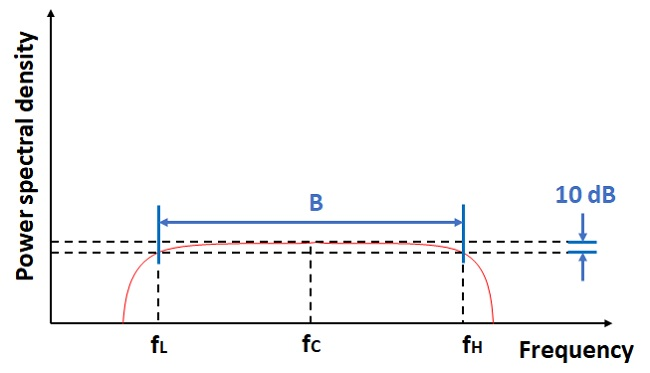
\includegraphics[width=\linewidth]{graphics/UWB_spectrum.jpg}
\caption{Power Spectral Density: Bandwidth B, lower-frequency f\textsubscript{L}, upper-frequency f\textsubscript{H}, \cite{hsu_2021}}
\label{f:UWB_spectrum}
\end{figure}


\subsubsection{UWB supported Nodes}

The IEEE 802.15.4 standard distinquishes between two types of devices.
Full-function device (FFD) are capable of connecting to multiple other devices, receive, transmit and coordinate. Reduced-function device (RFD) on the other hand can only connect to one other device and act as worker. 
In Topological terms RFDs can only operate as leaves, while FFDs can be any node in a network, including leaves.
RFDs therefore are strictly worse, but make up for it by requiering fewer resources, such as memory and power.
When FFDs work as PAN coordinators, they can use short adresses to address any node.
The PAN also has a PAN identifier, to help communication accross multiple networks, while still using the short address.
Each device also has a extended address, that is not assigned by any coordinator, that serves as a universal unique identifier (UUID).


\subsection{UWB MAC}
\label{sec:UWB MAC}

The Mac Layer is part of the Data link layer.
The Mac Frame is the payload of the PHY frame. It carries information about the type of frame, frame-format, security mechanism, adressing and frame validation.
The Mac Layer additionaly provides rules for beacon managment, chanel access.

\begin{figure}[ht!]
	\centering
	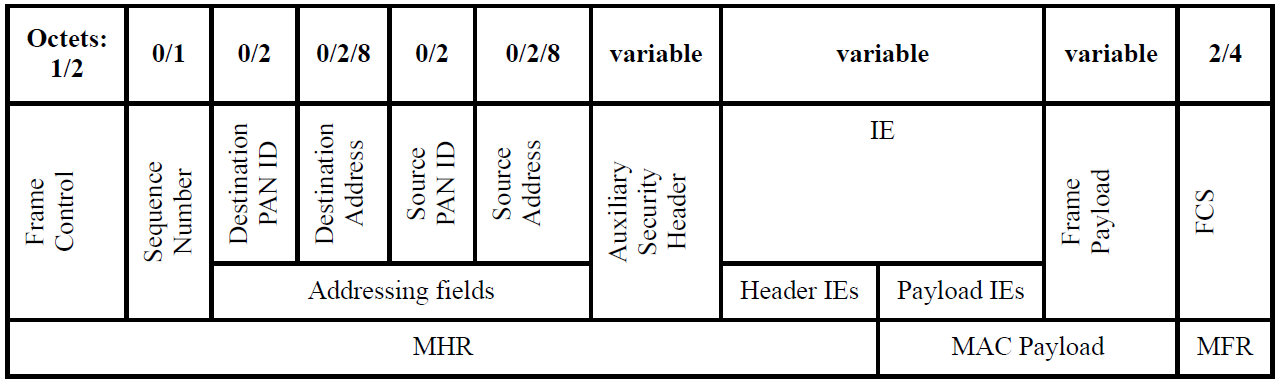
\includegraphics[width=\linewidth]{graphics/general_MAC_Frame_Format.png}
	\caption{General MAC Frame Format \cite{IEEE4-2020-7}}
	\label{f:MAC Frame Format}
\end{figure}


\subsubsection{MAC Frame Format}

Figure \ref{f:MAC Frame Format} shows the composition of a UWB-MAC frame.

In the MAC header (MHR), the Frame Control Field includes information about:

\begin{itemize}
  \item the frame-type
  \item if the Auxiliary Security Header Field is used and in what capacity
  \item if additional frames will follow
  \item if an acknowledgment message is expected
  \item if the message is between different PAN-Networks.
  \item of what type the receiver is (PAN coordinator, device, PAN-Network)
  \item the used frame-format standard
  \item where to find the source address
\end{itemize}

The Sequence Number counts up, helping to keep track of the order in which frames arive.
The Adressing Fields carry the IDs of sender and recipient for the frame.
The Auxiliary Security Header Field only exists if it was specified in the control Field.
It contains additional information needed for the chosen security methode.

There are two parts to the information element (IE).
The header IE specifies additional information about the frame, for example data formating information or chanel time allocation.
The the payload IE specifies the length and data-type of the payload field.
The payload containes the data that is sent.
It and the IE are of variable length, depending of the frame-type and data-length.

The MAC footer (MFR) marcs the end of the frame.
It only contains the frame checking sequence (FCS), that can be used to detect corrupted frames using cyclic redundancy checks.

\subsection{UWB PHY}

\subsubsection{PHY Chanel}

The IEEE 802.15.4z amendment defines 16 channels for communication for HRP UWB. 
A chanel is defined by its center frequency.
UWB devices can transmit on three different bands, high band, low band and sub-gigahertz.
For each band their is one chanel that is mandatory to support, if a device suports the band.
The other channels are optional, but if two devices want to communicate with each other they need to use the same band.
The bands, 16 chanels and their ranges and which chanels are mandatory can be found in table  (see table \ref{Table:: UWB frequency and channel assignments}).


\begin{table}[ht!]
\centering
\begin{tabular}{|l|l|c|c|}
\hline
\textbf{Channel number} & \textbf{Center frequency (MHz)} & \textbf{HRP UWB band}       & \textbf{Mandatory}  \\ 
\hline
0                       & 499.2                           & sub-gigahertz               &  \checkmark     \\ 
\hline
1                       & 3494.4                          & \multirow{4}{*}{Low band}   &                   \\ 
\cline{1-2}\cline{4-4}
2                       & 3993.6                          &                             &                   \\ 
\cline{1-2}\cline{4-4}
3                       & 4492.8                          &                             & \checkmark      \\ 
\cline{1-2}\cline{4-4}
4                       & 3993.6                          &                             &                   \\ 
\hline
5                       & 6489.6                          & \multirow{11}{*}{High band} &                 \\ 
\cline{1-2}\cline{4-4}
6                       & 6988.8                          &                             &                   \\ 
\cline{1-2}\cline{4-4}
7                       & 6489.6                          &                             &                   \\ 
\cline{1-2}\cline{4-4}
8                       & 7488                            &                             &                   \\ 
\cline{1-2}\cline{4-4}
9                       & 7987.2                          &                             & \checkmark       \\ 
\cline{1-2}\cline{4-4}
10                      & 8486.4                          &                             &                   \\ 
\cline{1-2}\cline{4-4}
11                      & 7987.2                          &                             &                   \\ 
\cline{1-2}\cline{4-4}
12                      & 8985.6                          &                             &                   \\ 
\cline{1-2}\cline{4-4}
13                      & 9484.8                          &                             &                   \\ 
\cline{1-2}\cline{4-4}
14                      & 9984                            &                             &                   \\ 
\cline{1-2}\cline{4-4}
15                      & 9484.8                          &                             &                 \\
\hline
\end{tabular}
\caption{ HRP UWB Frequency and Channel Assignments  \cite{IEEE4-2020-7, IEEE4z}}
\label{Table:: UWB frequency and channel assignments}
\end{table}

\subsubsection{Scrambled timestamp sequence}

The 4z amendment added the option to include a scrambled timestamp sequence (STS) into the frame.
The STS is a cyphered sequence that includes the timestamp and is used for ranging.
It is ment to increase the accuracy and integrtity of the raging results.
Before transmition receiver and sender exchange a randomly generated key.
The key is then used to encrypt the timestamp using the advanced encryption standard (AES) with 128 bits.
This ensured that the signal has not been intersepted and changed, to manipulate the ranging result.
Devices that support STS are called HRP-enhanced ranging capable
devices (HRP-ERDEV).

\subsubsection{Pulse Repetition Frequency}
\label{sec:pule repetition frequency}
The pulse repetition frequency (PRF) is the frequency at wich bursts are sent by the transmitter.
The mean PRF is the average PRF while sending the payload (power switching service data unit PSDU). %https://www.keysight.com/blogs/en/tech/rfmw/2021/07/28/an-overview-of-the-ieee-802154-hrp-uwb-standard
The higher the mean PRF, the shorter the airtime of each frame and allows for faster communication.
HRP-ERDEV use a different mean PRF than general devices.
They can work in Base pulse repetition frequency (BPRF) operating at mean PRF 64 MHz or in higher pulse repetition frequency (HPRF) mode operating above BPRF (Table \ref{f:mean PRF}).

\begin{table}[ht!]
\centering
\begin{tabular}{|l|l|l|} 
\hline
\textbf{Standard}          & \textbf{HRP UWB mode} & \textbf{mean PRF}            \\ 
\hline
802.15.4                   & Non HRP ERDEV         & 3.9 MHz, 15.6 MHz, 62.4 MHz  \\ 
\hline
\multirow{2}{*}{802.15.4z} & HRP-ERDEV BPRF        & 62.4 MHz                     \\ 
\cline{2-3}
                           & HRP-ERDEV HPRF        & 124.8 MHz, 249.6 MHz         \\
\hline
\end{tabular}
\caption{HRP UWB Mean PRF (Based on IEEE 802.15.4 and IEEE 802.15.4z, \cite{IEEE4-2020-7, IEEE4z})}
\label{f:mean PRF}
\end{table} %cite euse eigeni bricht

\subsubsection{Symbol Encoding}
UWB sends symbols by transmitting a burst of pulses that encode the symbol.
Since the pulses have clean edges, the arival time can be measured precisly.
This leads to the burst having two ways to carry information( \cite{QorvoGettingBacktoBasics}):
\begin{itemize}
  \item Binary phase-shift keying (BPSK: Encoding zeros and ones shifting the pulses phases so the burst beak for one has an oposite amplitude to the other. 
Figure \ref{f:UWB_signal_description} shows the singal 101 binary phase-shift keyed. 
Each bit is set twice, to detect problems with transmission.
  \item Burst position modulation (BPM): Changing the timing of the burst so it falls into a different time-slot inside of the possible burst position.	
Figure \ref{f:symbol structure} shows how the burst can be placed in a BPM-interval. 
The burst can't be placed in the guard interval. 
The guard exists to minimize inter-symbol interference from the
signals taking multiple paths.
\end{itemize}

\begin{figure}[ht!]
	\centering
	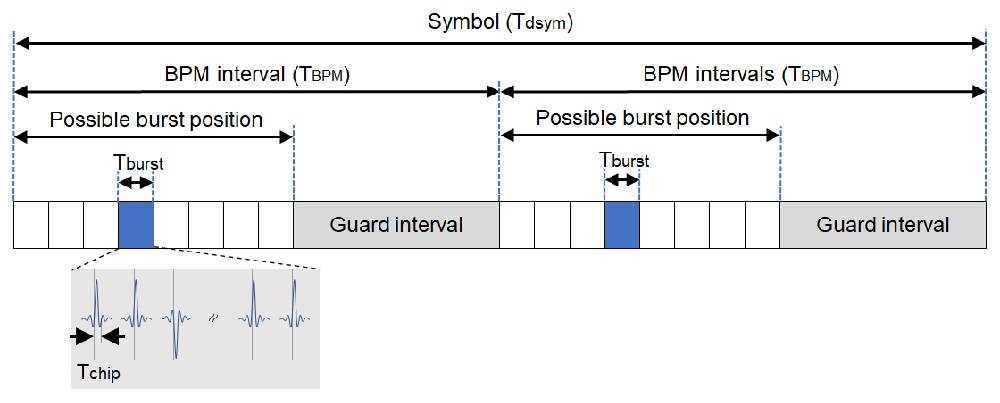
\includegraphics[width=\linewidth]{graphics/HRP_UWB_PHY_symbol_structure.jpg}
	\caption{HRP UWB PHY Symbol Structure \cite{hsu_2021}}
	\label{f:symbol structure}
\end{figure}

One or both of these encoding-strategies can be used in a uwb transmission.
The poition of the pulses inside of the burst (see figure \ref{f:UWB_signal_description})  relative to each other can be used to detect the presence of multipath effects and adjust for them. 
Using this, precises arrival times for the whole signal can be calculated.

\begin{figure}[ht!]
	\centering
	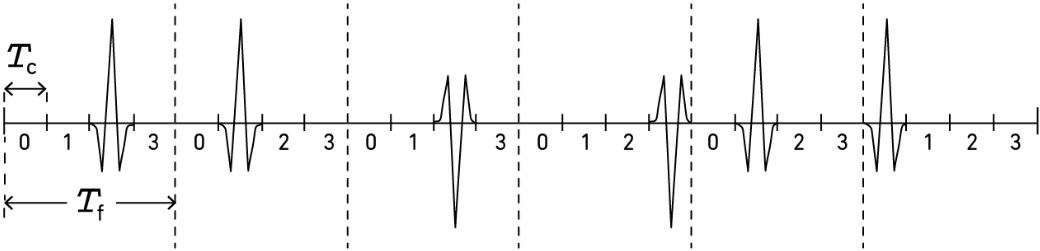
\includegraphics[width=\linewidth]{graphics/uwb_signal_tramsmission.png}
	\caption{UWB signal transmission byte encoding, \cite{QorvoGettingBacktoBasics}}
	\label{f:UWB_signal_description}
\end{figure}

Non-HRP ERDEV use BPM and BPSK.
Some HRP-ERDEV can use only BPSK, using a higher PRF and therefore reducing airtime.








\subsubsection{PHY Frame}
Figure \ref{f:PPDU general} shows a schematic view of a PHY frame as defined by the IEEE 802.15.4 standard.
The Synchronziation header (SHR) containes the information needed to detect the signal and ajust to its parameters.
The PHY header contains meta information about the payload and its encoding.
The PHY payload contains the data that is to be send, namly the MAC frame.

\begin{figure}[!ht]
\centering
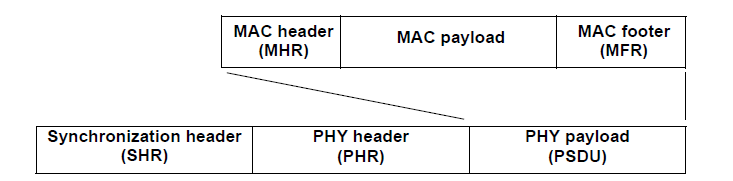
\includegraphics[width=\linewidth]{graphics/Schematic_view_PPDU.png}
\caption{Schematic view of a PHY frame defined by IEEE 802.15.4 \cite{IEEE4-2020-7}}
\label{f:PPDU general}
\end{figure}


Figure \ref{f:SHR field} shows the synchronization header, consiting of two parts.
The SYNC section is detectable by the receiver and informs it that a transmission has started.
Depending on the predefined mode, pulses of different length.
The sequence of pulses specify a set of chanels that can be used for communication.
The preamble can also be used to identify a PAN coordinator.

The SHR ends with the Start of Frame Delimiter (SFD).
It indicates that the synchronization has ended and the comming signals will be data, starting with the PHY header. 
It also contains a timestamp which can be used for ranging using time difference of arrival (ToA), see section \ref{TODO: put in this section}


\begin{figure}[!ht]
\centering
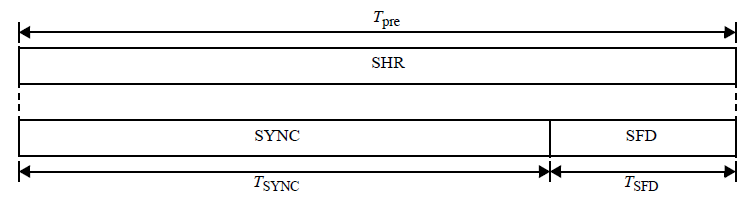
\includegraphics[width=\linewidth]{graphics/SHR_field_structure.png}
\caption{SHR Field Structure \cite{IEEE4-2020-7}}
\label{f:SHR field}
\end{figure}	

The PhY header contains all information needed to read the PHY payload (see Figure \ref{f:PHR general}).
The first bit defines the data rate that will be used during the playload transfer (see section \ref{sec:pule repetition frequency}).
The next seven bits define the length of the frame, with a frame length of maximal 128 bytes.
the 10th bit shows if ranging will be used with this frame.
The next bit is reserved.
Bits 11 and 12 define the preamble duration. It specifies how many repetitions are used, which can range from 16 to 4096.
The last 6 bits are single error correct, double error detect (SECDED) bits that form a Hammock block and can be used to correct single bit errors and detecting, but not fixing, double bit errors.

The last part of the PHY frame is the The PHY payload (PSDU).
This contains the the MAC frame, as defined in section \ref{sec:UWB MAC}.

\begin{figure}[ht!]
\centering
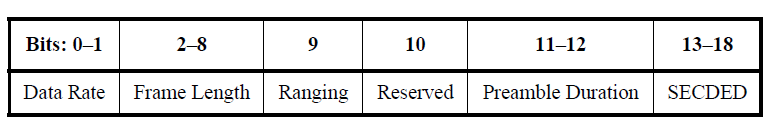
\includegraphics[width=\linewidth]{graphics/PHR_field_format_4.png}
\caption{General PHR Field Format \cite{IEEE4-2020-7}}
\label{f:PHR general}
\end{figure}

The 802.15.4z amendment contains optional changes to the PHY frame format if the participaiting devices are HRP-ERDEV devices.
Figure \ref{f:HRP-erdev frame} shows the newly allowed structures for a UWB frame.
Configuration 1 is equivalent to the already existing PHY frame.
The others additionaly contain a scrambled time stamp.
This can be placed in different places after the SHR.
Since UWB can also be used only for ranging without transmitting a message, configuration 3 only contains the SHR and STS, without a payload.

\begin{figure}[ht!]
\centering
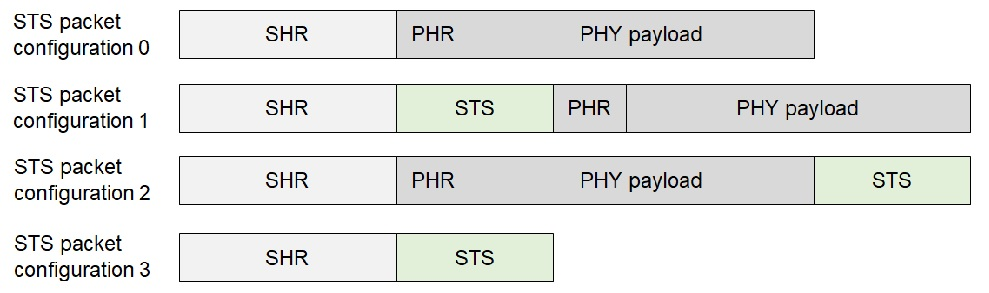
\includegraphics[width=\linewidth]{graphics/HRP_ERDEV_frame_structures.jpg}
\caption{HRP-ERDEV Frame Structures \cite{hsu_2021}}
\label{f:HRP-erdev frame}
\end{figure}

Additionally the PHR can be formatted differently (see gigure \ref{f:PHR 4z}. 
The reserved field and preamble duration is removed to make more space for the frame length. This allows to send more data in one frame, increasing the throughput of the UWB communication.

\begin{figure}[ht!]
\centering
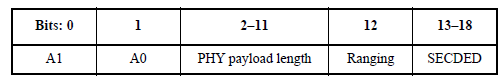
\includegraphics[width=\linewidth]{graphics/HRP_ERDEV_HPRF_mode_PHR.png}
\caption{PHR Field Format for HRP-ERDEV in HPRF Mode \cite{IEEE4z}}
\label{f:PHR 4z}
\end{figure}


\subsection{Two-way ranging}
\label{ss:two_way_ranging}
The IEEE 802.15.4z UWB standard describes two ranging methods, single-sided two-way ranging (SS-TWR) and Double-sided two-way ranging (DS-TWR).
In both instances, the distance measurement is done by calculating the time of flight (ToF) of a signal sent between two device using timestamps and multiplying it with the speed of light. 
In this section both SS-TWR and DS-TWR will be discussed.
In all other parts of the thesis,two-way ranging(TWR) refers to DS-TWR.

\textbf{Single-sided two-way ranging (SS-TWR)}:
During  SS-TWR, one device sends a message to a second and measures the round-trip time (see figure \ref{f:ss_twr}).
Device A sends a message to B and records a timestamp when the message was sent, $T_{A0}$.
When device B receives the respondes, it also records a timestamp, $T_{B0}$.
After some delay device B will send a response to A, that contains $T_{B0}$ and the current timestamp $T_{B1}$.
Device A on receiving the response records its timestamp, $T_{A1}$.
The round trip time $T_{round}$ can now be calculated using the timestamps from A:
\begin{equation}
	\mbox{$T_{round}$} =
	\mbox{$T_{A1} - T_{A0}$}
\end{equation}
The reply delay $T_{reply}$ is calculated using the timestamps from B:
\begin{equation}
	\mbox{$T_{reply}$} =
	\mbox{$T_{B1} - T_{B0}$}
\end{equation}

The ToF can be calculated by subtracting these values.
Since the messages was send the same distance twice, the ToF needs to be halved before multiplying it with the speed of light, to get the distance.
\begin{equation}
	\mbox{$distance$} =
	\mbox{$(\frac{1}{2}\cdot T_{round}-T_{reply}) \cdot c_{air}$}
\end{equation}

\begin{figure}[ht!]
\centering
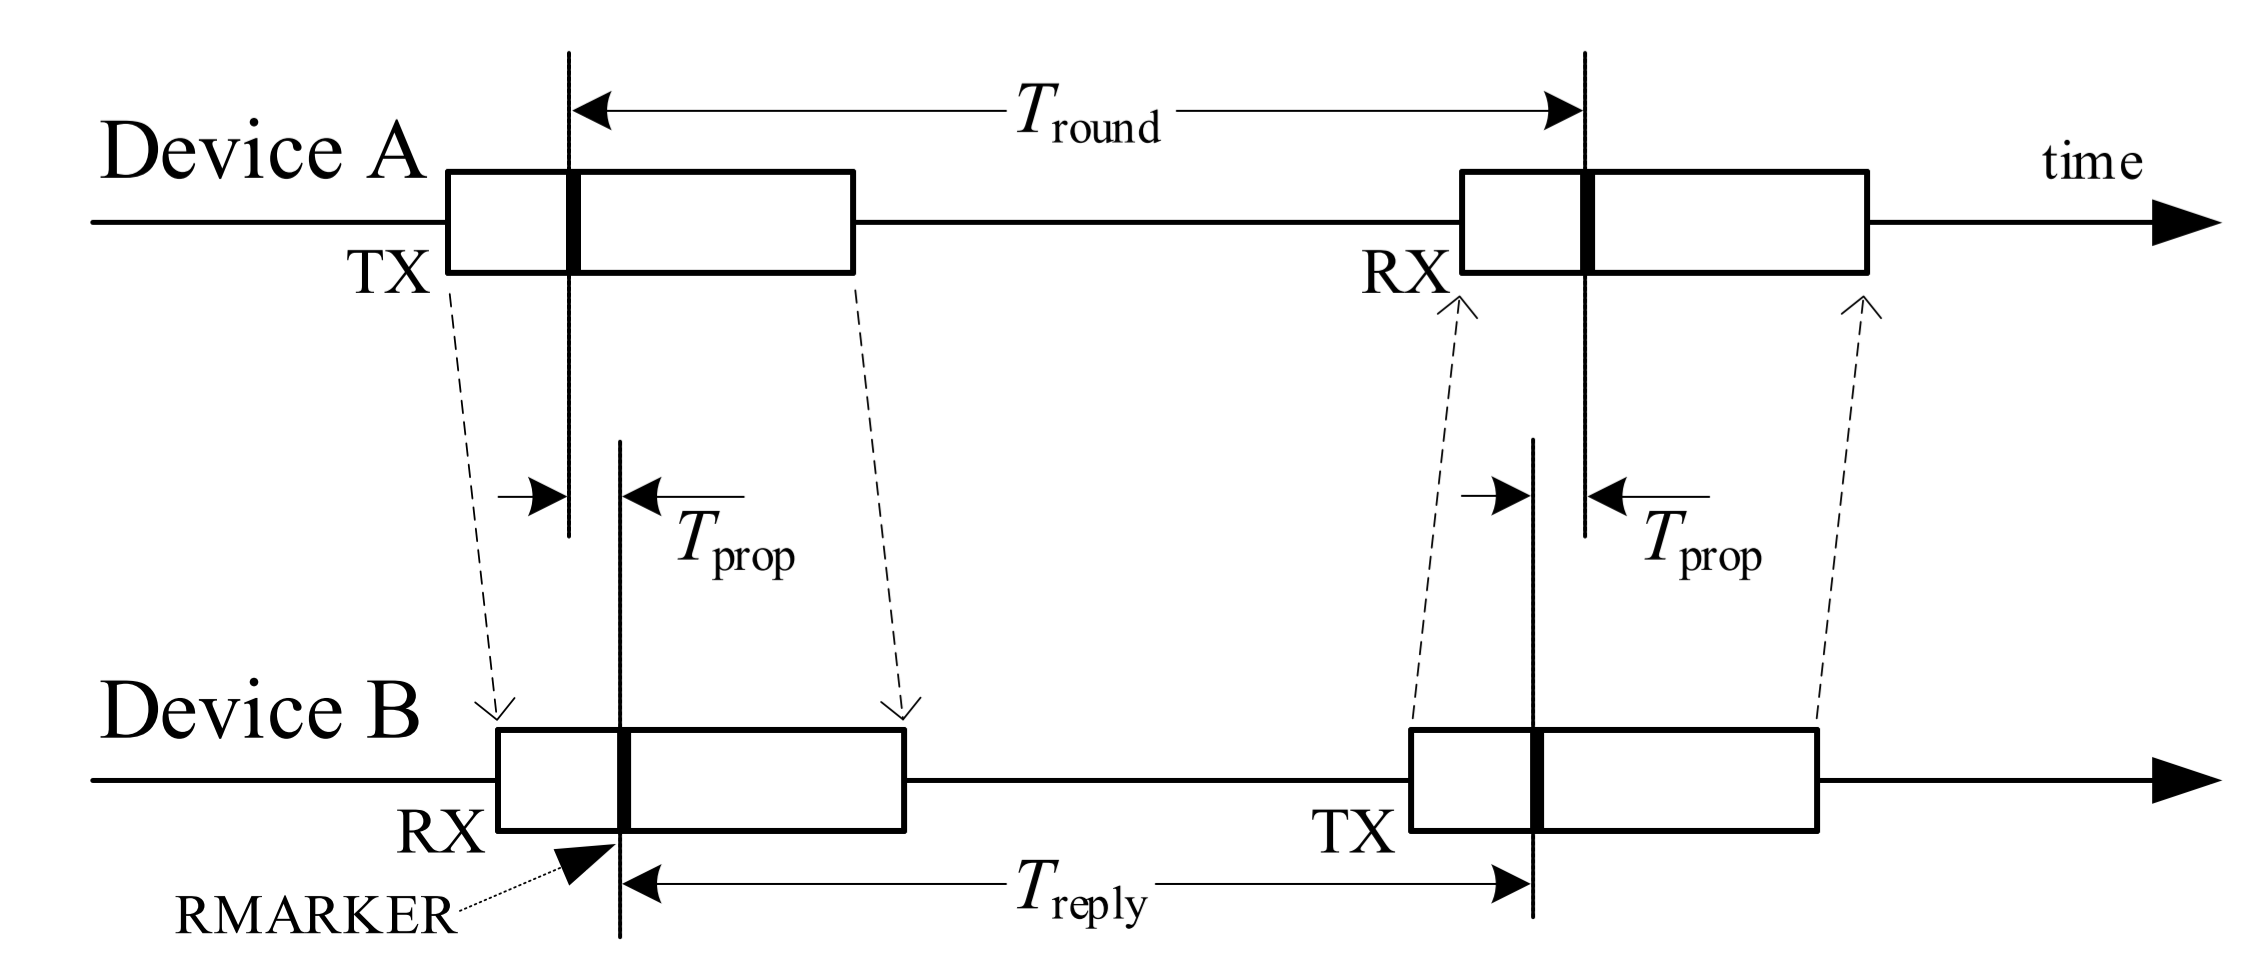
\includegraphics[width=\linewidth]{graphics/schematics/SingleSidedTwoWayRanging.png}
\caption{timeline of singe-sided two-way ranging (SS-TWR)\cite{IEEE4z}}
\label{f:ss_twr}
\end{figure}

\textbf{Double-sided two-way ranging (DS-TWR)}:
In DS-TWR involves both device A and B performing a SS-TWR and calculating the average between the results.
Figure \ref{f:ds_twr} shows the two seperate ranging sessions.
Their result can then be combined to the average ToF for a single message:
\begin{equation}
	\mbox{$T_{prop}$} =
	\mbox{$\frac {T_{Round1}\cdot T_{Round2}-T_{Reply1}\cdot T_{Reply2}}{T_{Round1}+T_{Round2}+T_{Reply1}+T_{Reply2}}$}
\end{equation}
\begin{equation}
	\mbox{$distance$} =
	\mbox{$T_{prop} \cdot c_{air}$}
\end{equation}

The two ranging sessions can have one message overlapping.
Figure \ref{f:ds_twr_3}} shows the timeline of an overlapping DS-TWR that only requires three messages.

\begin{figure}[ht!]
\centering
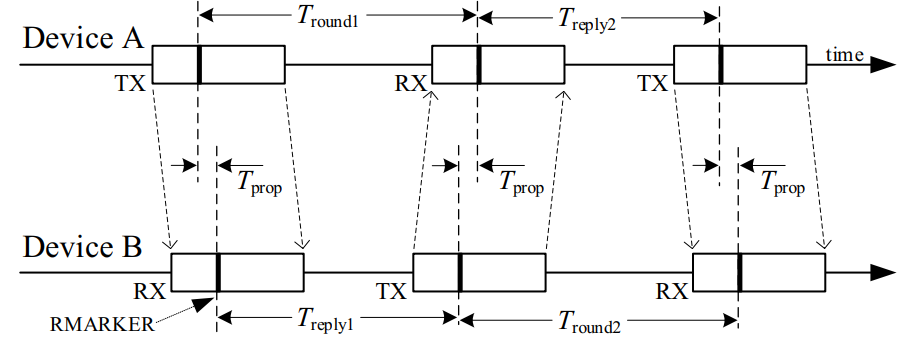
\includegraphics[width=\linewidth]{graphics/schematics/TwoSidedRangingThreeMessages.PNG}
\caption{timeline of singe-sided two-way ranging (SS-TWR) with three messages\cite{IEEE4z}}
\label{f:ds_twr_3}
\end{figure}


\begin{figure}[ht!]
\centering
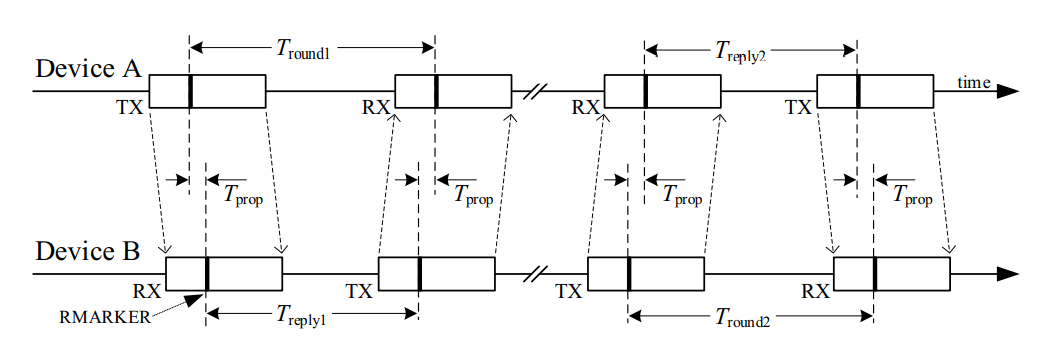
\includegraphics[width=\linewidth]{graphics/schematics/TwoSidedTwoWayRanging.PNG}
\caption{timeline of double-sided two-way ranging (DS-TWR)\cite{IEEE4z}}
\label{f:ds_twr}
\end{figure}

\section{Related Work} % application of concepts


\subsection{Artwork Tracking}


Since art preservation is an old field and temperature, humidity, light and vibrations have been known to be detrimental to most artworks, especialy paintings, most research in this direction is older than 20 years \cite{mecklenburg1991mechanical, michalski1991paintings, saunders2004effect}.
Still, the envention of new technologies, such as pattern recognizion using artificial inteligence, improvement on existing tools like infrared imaging and a active need for solutions have kept the resaech into artwork preservation an active field \cite{borg2020application, schito2017integrated}.
One such new technologies are sensor networks, which have become widespread in the field of art-preservation \cite{shah2016customized}.


Artwork tracking during transportation has not been a major focus in academia.
The most relevant related research was done by Fort et al. \cite{landi2022iot}.
They developed a low-cost, low powered sensor node to track temperature, humdity, pressure and vibrations of artwork and wooden structures.
The sensor node would then report its findings to a remote server.
They confirmed the validity of their sensor in a series of experiments, that were performed in a static building.
They also presented a theoretical framework for their sensor to be used in a transportation scenario, but they do not report having implemented or tesed this system.
Their sensor used an ascelerometer to detect vibrations, and the Bosch BME280 sensor to detect pressure, temperature and humidity.
Their sensors did not build a network and were not queried, but reported their findings directly to either a wlan router or a ble-capable smart-device.
The research of Fort et al. showed the value of low-cost sensors in the detection of threats to artwork.

\subsection{Sensor Networks}

Wireless Sensor Networks (WSN) have become a central aspect if IoT.
Researchers have tried to focus on the most prevelant problems arrising from the development of NSWs, mainly power managment, security and privacy, data integrity and avaliability \cite{gulati2022review}.


\cite{garg2021healthcare} researched WSNs outside of the controlled environment of a house. They propose a WSN that can track thevitals of mountainiers and call for help when measurements have dangerous values. 
They used an Ardruino Mega board equiped with a radio transiever, using LoRa with a star-topology, was used.


\cite{jones2021wireless} created a WSN of NRF24101 board that is intended to monitor linear infrastructures like deepsee wires, using radio and wifi for communication. Using deep sleep they were able to optimize energy usage so the sensor is predicted to last five years on batery.


\cite{spandonidis2022evaluation} used an acelerometer to detect vibrations in pipeline to discover leaks. 
They used a narrowband connection for communication and GPS for localization.
Their sensors could query each other for data, to provide a more complete image of the situation.


\subsection{Wireless ranging}

\cite{li2024indoor} made an overview of publications envolving positioning systems for industrial settings. 
They looked at the positioning systems in papers using RFID, BLE, UWB, Wi-Fi and ZigBee. They found that UWB consistently reported the highest accuracy of these methods.
UWB was the least affected by multipath-effects, although it was still the most common issue with this technology.


Early research of ranging using UWB was done by Gezici et al. \cite{gezici2008survey, gezici2005localization}.
These papers gave an overview of the different positioning systems for UWB, angle of arival, recived signal strength, time of arrival and time difference of arival.
Time of arival and time difference of arrival were studied further in these publications, presenting errorsources and mitigation tools.


Early research focused on augmentation of UWB ranging methods.
\cite{venkatesh2007nlos} proposed using integer programs for midigating the error for ranging without line-of-sight.
\cite{guvencc2007nlos} tried to solve the same issue by using methods based on the statistics of multipath-effects.
BiasSub and BiasRed was proposed to reduce the bias in time difference of arival, by appling of a well-known algebraic explicit solution for source localization  \cite{ho2012bias}.
\cite{fan2017performance} emproved uwb ranging by eliminating random error. They did this by pre-filtering, using a anti-magnetic ring to eliminate outliers and using the double-state adaptive Kalman filter to improve position accuracy.
Newer research has also begone incorporating neural networks into UWB positioning systems \cite{stahlke2020nlos, ridolfi2021uwb, che2020machine}.

UWB localization has been used in many applied context.
It has been proposed for pedestrian tracking \cite{otim2019effects}, drone flying \cite{macoir2019uwb},robot navigation \cite{zhu2020adapted}, navigation system for visualy impared people \cite{rosiak2024effectiveness} and tracking people in buildings \cite{elbaum2024investigating}.
UWB positioning systems are particularly interesting for industrial IoT settings.
\cite{barbieri2021uwb} measured the performance of three different UWB antennas, Qorvo, Sewio, and Ubisense. They measured a lot of multiplath-effects in such a complex environment. The midigated this by employing a Bayesian filtering method.
\cite{belli2024cloud} used UWB positioning in combination with Real-time kinematic positioning, to track workers while monitoring the factory. The goal was to trigger an alarm if a dangerous situation occured.
